\documentclass{beamer}
%Information to be included in the title page:
\title{Digital Tools Project-Effect of Interest Rate Changes on Cryptocurrencies.}
\author{Cameron Storey, Marc David Parker, Matthias Olieslagers, Qian Chen}

\institute{UZH Digital Tools for Finance}
\date{2022}



\begin{document}

\frame{\titlepage}

\begin{frame}
\frametitle{Introduction}
In this project we aim to analyse the effect of FED rate changes on the price of BTC and also the price action.\\


We will look at multiple methods and see if there are any significant results with an aim to create a strategy we could use to successfully trade cyrptocurrency markets.
\end{frame}

\begin{frame}
    \frametitle{Our Code}
    The code we have developed within Python, we have used a range of python packages as follows:
    \begin{itemize}
    \item Pandas
    \item Numpy
    \item matplotlib
\end{itemize}
The following were used for our data handling, data analysis and our data visualisation.
\end{frame}

\begin{frame}
    \frametitle{Findings, n day change}
We ran multiple methods the fist was an analysis of the price change n days after a FED rate change. We were looking to see if there is a significant move on a specific day. \\
\begin{center}
    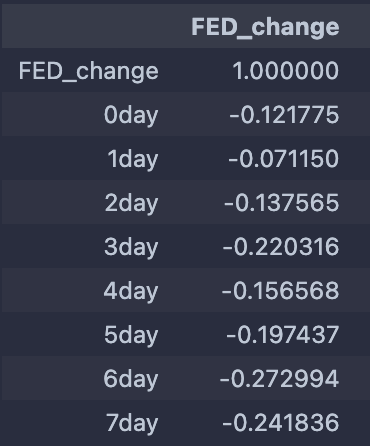
\includegraphics{research_project/text/paper/1.png}
\end{center}


\end{frame}
\begin{frame}
    \frametitle{Findings, n day change}
We see no significant evidence of a price change in a certain direction on a specific day. So we will now perform a moving average analysis.
\end{frame}

\begin{frame}
    \frametitle{Findings, Moving Average}
As we observed no significant result we have moved onto Moving average in which we obtained the following data/results.
\begin{center}
  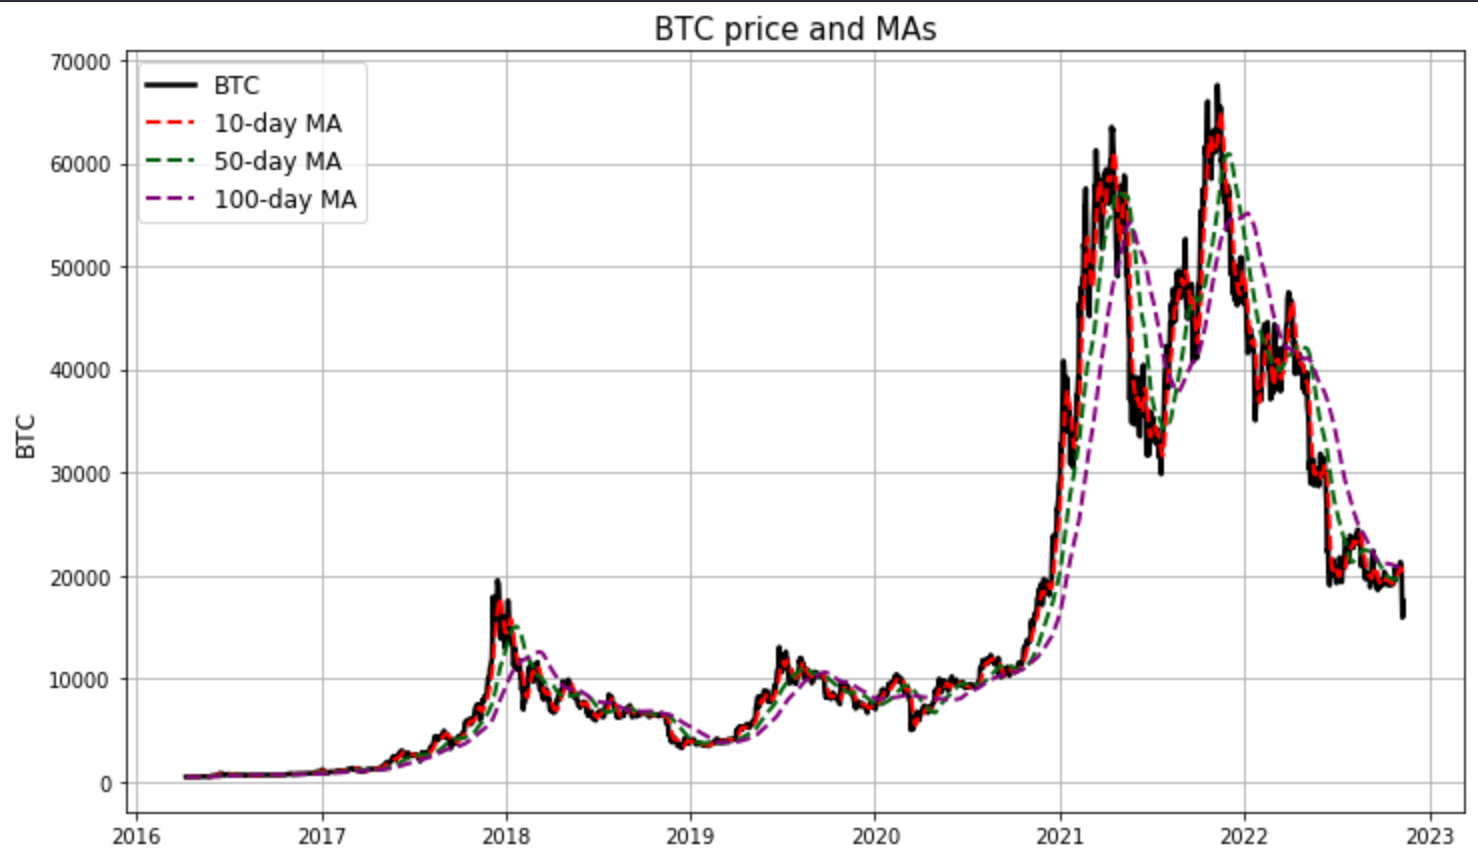
\includegraphics[width=0.5\textwidth]{research_project/text/paper/2.png}
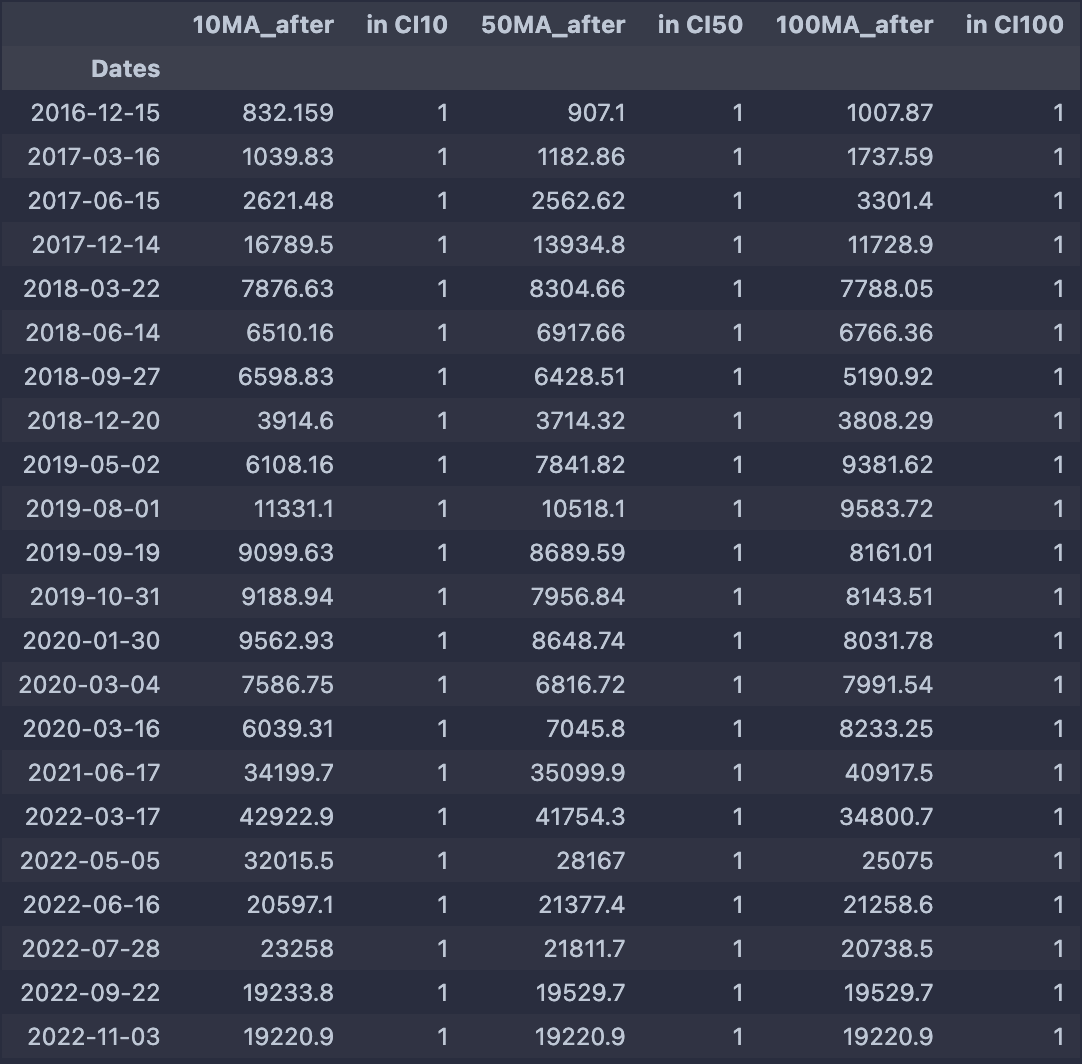
\includegraphics[width=0.5\textwidth]{research_project/text/paper/3.png}  
\end{center}
\end{frame}

\begin{frame}
    \frametitle{Findings, Moving Average}
Once again we see nothing significance so we will move onto volatility analysis.
\end{frame}

\begin{frame}
    \frametitle{Findings, Volatility}
We now chose to analyse if there is any effect on the volatility and daily change of the BTC price data when there is a FED rate change.
\begin{center}
 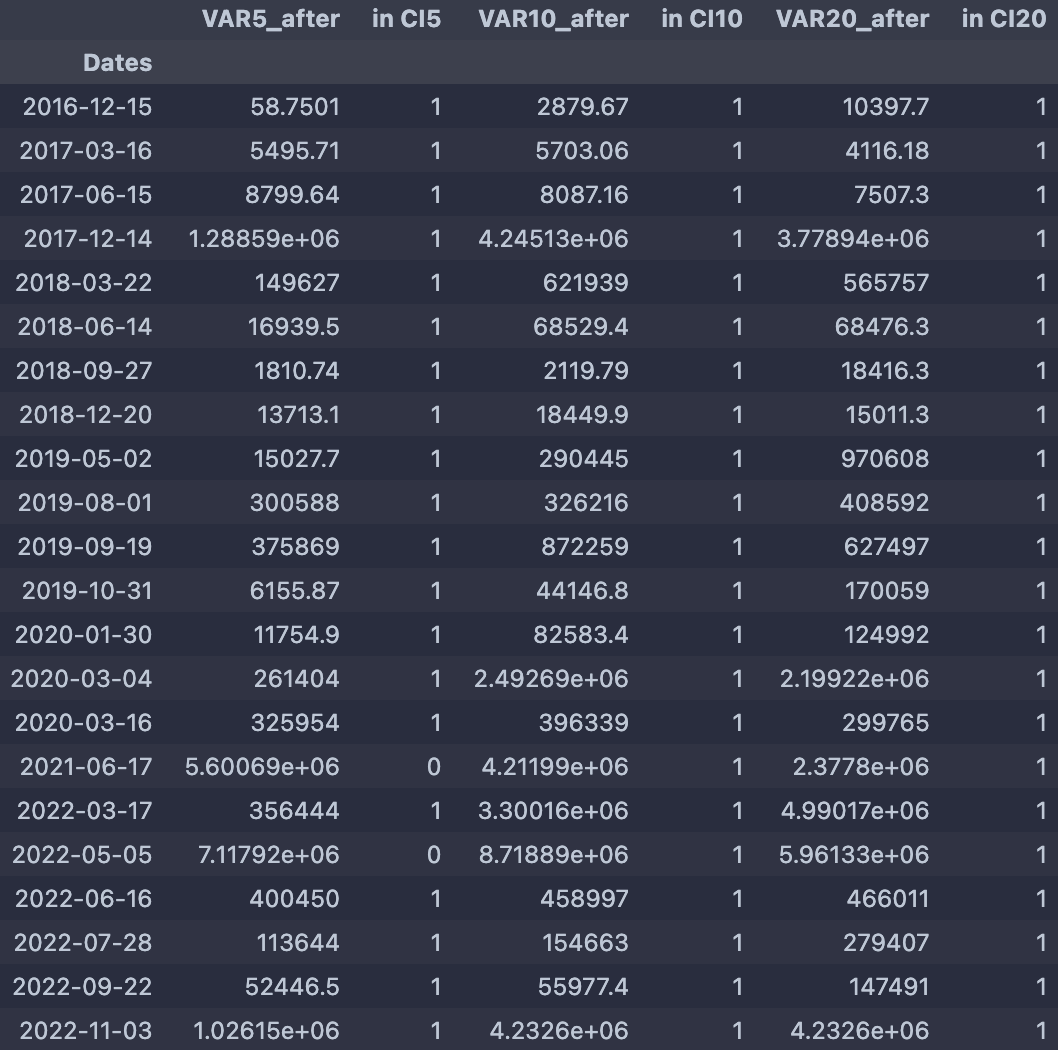
\includegraphics[width=0.5\textwidth]{research_project/text/paper/7.png}

\end{center}

\end{frame}
\begin{frame}
    \frametitle{Findings, Volatility}

\begin{center}
 
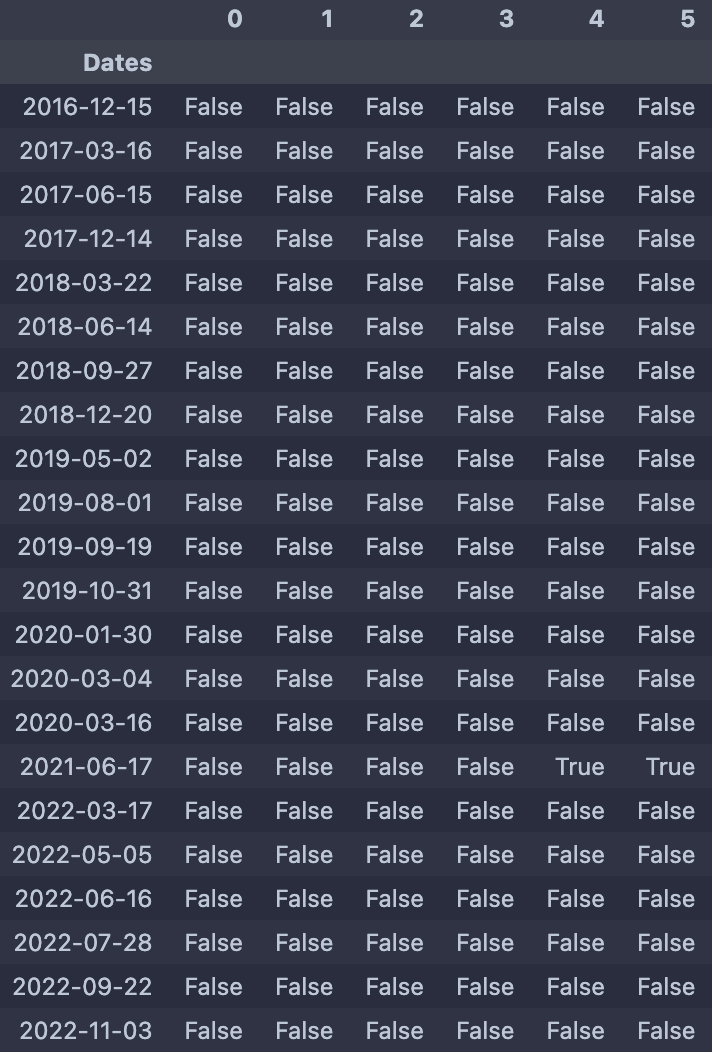
\includegraphics[width=0.5\textwidth]{research_project/text/paper/10.png}     

\end{center}

\end{frame}

\begin{frame}
    \frametitle{Findings, Volatility}
Once again we see the FED rate change has no significant effect of the BTC price change or price Action, we see some significant results but we do not believe this is due to the FED changing the rate and more likely because of something else happening in the world and the market.
\end{frame}

\begin{frame}
    \frametitle{Conclusion}
    In conclusion we do not believe, there is a significant effect of FED rate changes on the price of BTC. So we are unable to come up with a profitable trading strategy based on FED rate change and FED announcements alone. 
\end{frame}

\end{document}